%% LyX 2.3.4.2 created this file.  For more info, see http://www.lyx.org/.
%% Do not edit unless you really know what you are doing.
\documentclass[english,dvipsnames,aspectratio=169,handout]{beamer}
\usepackage{mathptmx}
\usepackage{eulervm}
\usepackage[T1]{fontenc}
\usepackage[latin9]{inputenc}
\usepackage{babel}
\usepackage{amstext}
\usepackage{amssymb}
\usepackage{graphicx}
\usepackage{ifthen}
\usepackage{xcolor}
\usepackage{xspace}
\usepackage{tikz}
\usetikzlibrary{tikzmark}
\usetikzlibrary{calc}
\usepackage{pgfplots}
%\pgfplotsset{compat=1.17}
\usepackage{booktabs}
\usepackage{xpatch}
\usepackage{multirow}
\usepackage{colortbl}
\usepackage{pgfpages}


\xpatchcmd{\itemize}
  {\def\makelabel}
  {\ifnum\@itemdepth=1\relax
     \setlength\itemsep{2ex}% separation for first level
   \else
     \ifnum\@itemdepth=2\relax
       \setlength\itemsep{1ex}% separation for second level
     \else
       \ifnum\@itemdepth=3\relax
         \setlength\itemsep{0.5ex}% separation for third level
   \fi\fi\fi\def\makelabel
  }
 {}
 {}

\ifx\hypersetup\undefined
  \AtBeginDocument{%
    \hypersetup{unicode=true,pdfusetitle,
 bookmarks=true,bookmarksnumbered=false,bookmarksopen=false,
 breaklinks=false,pdfborder={0 0 0},pdfborderstyle={},backref=false,colorlinks=true,
 allcolors=NYUPurple,urlcolor=LightPurple}
  }
\else
  \hypersetup{unicode=true,pdfusetitle,
 bookmarks=true,bookmarksnumbered=false,bookmarksopen=false,
 breaklinks=false,pdfborder={0 0 0},pdfborderstyle={},backref=false,colorlinks=true,
 allcolors=NYUPurple,urlcolor=LightPurple}
\fi

\makeatletter

%%%%%%%%%%%%%%%%%%%%%%%%%%%%%% LyX specific LaTeX commands.
%% Because html converters don't know tabularnewline
\providecommand{\tabularnewline}{\\}

%%%%%%%%%%%%%%%%%%%%%%%%%%%%%% Textclass specific LaTeX commands.
% this default might be overridden by plain title style
\newcommand\makebeamertitle{\frame{\maketitle}}%
% (ERT) argument for the TOC
\AtBeginDocument{%
  \let\origtableofcontents=\tableofcontents
  \def\tableofcontents{\@ifnextchar[{\origtableofcontents}{\gobbletableofcontents}}
  \def\gobbletableofcontents#1{\origtableofcontents}
}

%%%%%%%%%%%%%%%%%%%%%%%%%%%%%% User specified LaTeX commands.
\usetheme{CambridgeUS} 
\beamertemplatenavigationsymbolsempty


% Set Color ==============================
\definecolor{NYUPurple}{RGB}{87,6,140}
\definecolor{LightPurple}{RGB}{165,11,255}


\setbeamercolor{title}{fg=NYUPurple}
\setbeamercolor{frametitle}{fg=NYUPurple}

\setbeamercolor{background canvas}{fg=NYUPurple, bg=white}
\setbeamercolor{background}{fg=black, bg=NYUPurple}

\setbeamercolor{palette primary}{fg=black, bg=gray!30!white}
\setbeamercolor{palette secondary}{fg=black, bg=gray!20!white}
\setbeamercolor{palette tertiary}{fg=gray!20!white, bg=NYUPurple}

\setbeamertemplate{headline}{}
\setbeamerfont{itemize/enumerate body}{}
\setbeamerfont{itemize/enumerate subbody}{size=\normalsize}

\setbeamercolor{parttitle}{fg=NYUPurple}
\setbeamercolor{sectiontitle}{fg=NYUPurple}
\setbeamercolor{sectionname}{fg=NYUPurple}
\setbeamercolor{section page}{fg=NYUPurple}
%\setbeamercolor{description item}{fg=NYUPurple}
%\setbeamercolor{block title}{fg=NYUPurple}

\setbeamertemplate{blocks}[rounded][shadow=false]
\setbeamercolor{block body}{bg=normal text.bg!90!NYUPurple}
\setbeamercolor{block title}{bg=NYUPurple!30, fg=NYUPurple}



\AtBeginSection[]{
  \begin{frame}
  \vfill
  \centering
\setbeamercolor{section title}{fg=NYUPurple}
 \begin{beamercolorbox}[sep=8pt,center,shadow=true,rounded=true]{title}
    \usebeamerfont{title}\usebeamercolor[fg]{title}\insertsectionhead\par%
  \end{beamercolorbox}
  \vfill
  \end{frame}
}

\makeatother

\setlength{\parskip}{\medskipamount} 

\input ../macros

\begin{document}
\input ../rosenberg-macros

%\setbeameroption{show notes on second screen}

\title[DS-GA 1003]{Decision Trees}
\author{He He  \\
Slides based on Lecture
\href{https://github.com/davidrosenberg/mlcourse/blob/gh-pages/Lectures/10.trees.pdf}{10} from David Rosenberg's course materials (\url{https://github.com/davidrosenberg/mlcourse})
}
\date{April 6, 2021}
\institute{CDS, NYU}

\makebeamertitle
\mode<article>{Just in article version}

\begin{frame}
{Today's lecture}
\begin{itemize}
\item Our first inherently non-linear classifier: decision trees.
\item Ensemble methods: bagging and boosting.
\end{itemize}
\end{frame}

\section{Decision Trees}

\subsection{Input Space Partition}

\begin{frame}
{Motivating example in 2d}
\begin{itemize}
%\item Decision tree is a \textcolor{blue}{non-linear} classifier
\item Partition data into different (axis-aligned) regions \textcolor{blue}{recursively}
\end{itemize}
\begin{center}
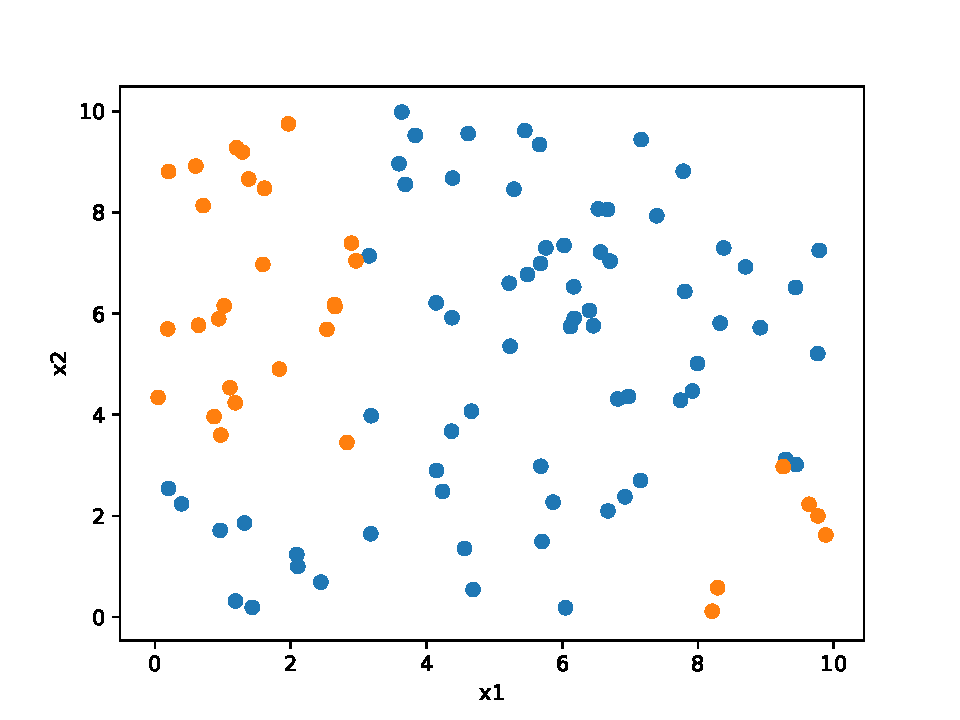
\includegraphics[height=0.6\textheight]{figures/dt-2d}
\end{center}
\note[item]{Let's consider the dataset shown in the figure. How should we classify the orange and the blue points?}
\note[item]{They are not linearly separable, but they belong to different regions. (draw regions)}
\note[item]{Let's partition the space recursively.}
\end{frame}

\begin{frame}
{Classification flowchart}
\begin{columns}
\begin{column}{0.5\textwidth}
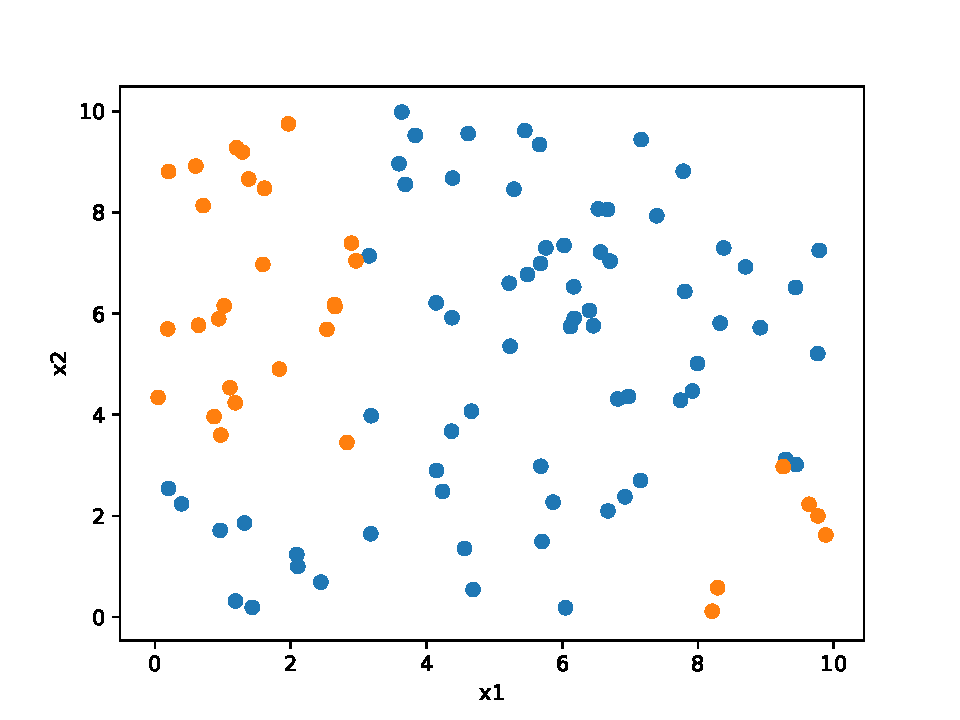
\includegraphics[height=0.6\textheight]{figures/dt-2d}
\end{column}
\begin{column}{0.5\textwidth}
\end{column}
\end{columns}
\onslide<2->{Is this a linear or non-linear classifier?}
\note[item]{(Draw partitions)}
\note[item]{The decision boundary is non-linear.}
\note[item]{How do we predict at test time? The prediction can actually be represented as a sequential decision process. (draw flowchart)}
\end{frame}

\begin{frame}
{Decision trees setup}
\begin{columns}
\begin{column}{0.5\textwidth}
\begin{center}
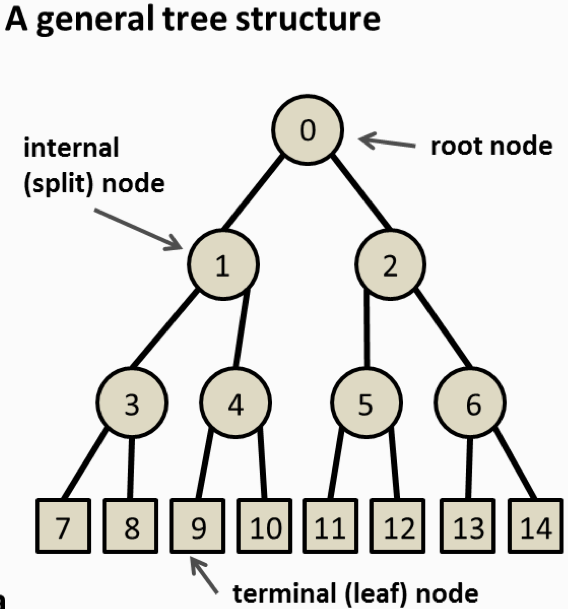
\includegraphics[height=0.7\textheight]{figures/generalTreeStructure}
\end{center}
\note<.>{Explain depth of a tree.}
\end{column}
\begin{column}{0.5\textwidth}
We'll only consider 
\begin{itemize}
\item \emph{binary} trees (vs multiway trees where nodes can have more
than 2 children)
\pause
\item each node contains a subset of data points
\pause
\item decisions at each node involve only a \emph{single} feature (i.e. input coordinate)
\item for continuous variables, splits always of the form 
\[
x_{i}\le t
\]

\item for discrete variables, partitions values into two groups
\end{itemize}
\end{column}
\end{columns}
\let\thefootnote\relax\footnotetext{\tiny{From Criminisi et al. MSR-TR-2011-114, 28 October 2011.}}

\note[item]{Let's review some terminology for trees you've probably seen in an algorithm class. We'll consider a rooted tree, where we have a designated root node. The nodes that have degree one (incident to only one edge) are terminal/leaf nodes. The other nodes are called internal nodes.}
\note[item]{Specifically, we'll consider binary trees where each node has two children.}
\note[item]{What does each node represent? They correspond to one partition of the data. The root node contains all data; we partition the data in one node by branching to its descendants.}
\note[item]{The branching decision at each node involves a single feature.}
\end{frame}

\begin{frame}
{Regularization of decision trees}
\begin{itemize}[<+->]
\item What will happen if we keep splitting the data?
\begin{itemize}
\item Every data point will be in its own region---\textcolor{red}{overfitting}.
\end{itemize}

\item When to stop splitting? (control complexity of the hypothesis space)
\begin{itemize}[<.->]
\item<+-> Limit number of total nodes.
\item Limit number of terminal nodes.
\item Limit tree depth.
\item Require minimum number of data points in a terminal node.
%\item \textbf{Backward pruning} -- the approach of \textbf{CART}
%(Breiman et al 1984): 
%\begin{enumerate}
%\item Build a really big tree (e.g. until all regions have $\le5$ points).
%\item \emph{Prune} the tree back greedily all the way to the root,
%assessing performance on validation.
%\end{enumerate}
\end{itemize}
\end{itemize}
\note[item]{A common approach in practice is backward pruning, similar to backward feature selection. The advantage is that we get the global view once the entire tree is built, where as in the other approaches we might stop too early and miss an important split that only comes later.}
\end{frame}

\begin{frame}
{How to split}
\begin{description}[<+->]
\item[Goal] Find a tree that minimize the task loss (\eg squared loss) within a given complexity.
\item[Problem] Finding the optimal binary tree is computationally intractable.
\item[Solution] \emph{Greedy} algorithm.
\begin{itemize}[<.->]
\item Find the best split (according to some criteria) for a non-terminal node (initially the root)
\item Add two children nodes
\item Repeat until a stopping criterion is reached (\eg max depth)
\end{itemize}
\end{description}
\note[item]{Given some stopping criteria, the next question is how do we find the split that will minimize our task loss in the end.}
\note[item]{In general, this is intractable.}
\note[item]{However, we can use a greedy algorithm to split each node in a locally optimal way, starting from the root.}
\end{frame}

\subsection{Node Splitting}
\begin{frame}
{Evaluate splits}
Let's think about what makes a good split.

\onslide<+->{
\begin{simpleblock}{Which one is better?}
\begin{description}
\item[Split 1] $R_1: 8+ / 2- \quad R2: 2+ / 8-$
\item[Split 2] $R_1: 6+ / 4- \quad R2: 1+ / 9-$
\end{description}
\end{simpleblock}
}
\onslide<+->{
\begin{simpleblock}{Which one is better?}
\begin{description}
\item[Split 1] $R_1: 8+ / 2- \quad R2: 2+ / 8-$
\item[Split 2] $R_1: 6+ / 4- \quad R2: 0+ / 10-$
\end{description}
\end{simpleblock}
}
\onslide<+->{
In general, we want to produce \emph{pure} nodes,
\ie close to single-class node.
}
\note[item]{Split 1 is better because it has low error rate.}
\note[item]{It's a bit tricky now. Both split has the same error rate. Note that in Split 2, R2 would be a terminal node already, so we might prefer Split 2; however, R1 still needs more work.}
\end{frame}

\begin{frame}
{Misclassification error in a node}
Let's formalize things a bit.
\begin{itemize}[<+->]
\item Consider classification case: $\cy=\left\{ 1,2,\ldots,K\right\} $.

\item What's in a node?
\begin{itemize}[<.->]
\item Let node $m$ represent region $R_{m}$, with $N_{m}$ observations
\item Denote proportion of observations in $R_{m}$ with class $k$ by
\[
\hat{p}_{mk}=\frac{1}{N_{m}}\sum_{\left\{ i:x_{i}\in R_{m}\right\} }\ind{y_{i}=k}.
\]
\end{itemize}

\item Predict the majority class in node $m$:
\[
k(m)=\argmax_{k}\hat{p}_{mk}.
\]

\item Misclassification rate in node $m$:
\[
1-\hat{p}_{mk(m)}.
\]
\end{itemize}

\note[item]{Each node contains a subset of data.}
\end{frame}

\begin{frame}{Node Impurity Measures}
How to quantify impurity?
\begin{itemize}[<+->]
\item Three measures of \textbf{node impurity} for leaf node
$m$:
\begin{description}[<+->][Misclassification error]
\item[Misclassification error]
\[
1 -  \hat{p}_{mk(m)}.
\]

\item[Gini index]
\[
\sum_{k=1}^{K}\hat{p}_{mk}(1-\hat{p}_{mk})
\]

\item[Entropy / Information gain]
\[
-\sum_{k=1}^{K}\hat{p}_{mk}\log\hat{p}_{mk}.
\]
\end{description}
\item Gini index and entropy work well in practice.

\note[item]{We would like a metric that gives high scores to nodes containing examples from many different classes, and low scores to nodes with few or a single class of examples.}
\note[item]{We've seen that the error rate can indicate node purity. When is it minimized? When $p$ is 1, i.e., all examples are in the same class. Note that this is different from the Gini index that measure inequality you might learn in economics.}
\note[item]{But it's not a ``sensitive'' measure. It's often the case that we will have many splits that gives the same misclassification error. Gini index is another popular metric. For each class $k$ we compute the product of the proportion of class $k$, $\hat{p}_{mk}$ and the other classes $1-\hat{p}_{mk}$. When is it minimized? $p=0 / 1$.}
\note[item]{Finally, we can use Shannon entropy, which measure the uncertainty of the label in this node. It's minimized when all labels are the same---no uncertainty.}
\note[item]{Both Gini index and entropy are information-theoretic measures.}

\end{itemize}
\end{frame}

\begin{frame}{Impurity of a split}
A potential split produces two nodes, $R_{L}$ and $R_{R}$.
How do we score it?
\begin{itemize}[<+->]
\item Suppose we have $N_{L}$ points in $R_{L}$ and $N_{R}$ points in
$R_{R}$.

\item Let $Q(R_{L})$ and $Q(R_{R})$ be the node impurity measures for each node.

\item Then find split that minimizes the \emph{weighted average of node
impurities}:
\[
\frac{N_{L}Q(R_{L})+N_{R}Q(R_{R})}{N_L+N_R}
\]
\end{itemize}

\onslide<+->{
\begin{simpleblock}{Example:}
$R_1: 8+ / 2- \quad R2: 1+ / 4-$\\
What's the weighted misclassification rate?
\end{simpleblock}
}
\note[item]{Now that we've defined impurity measure for a single node, how do we use it to evaluate a split, which produces two nodes?}
\note[item]{The weight is just the proportion of examples in left and right nodes.}
\note[item]{$Q_1 = 1/4, Q_2=1/4, w_1 = 10/15=2/3, w_2 = 1/3.$}
\end{frame}

\begin{frame}{\dis Two-Class Node Impurity Measures}
Consider binary classification. Let $p$ be the relative frequency of class 1.
\begin{figure}
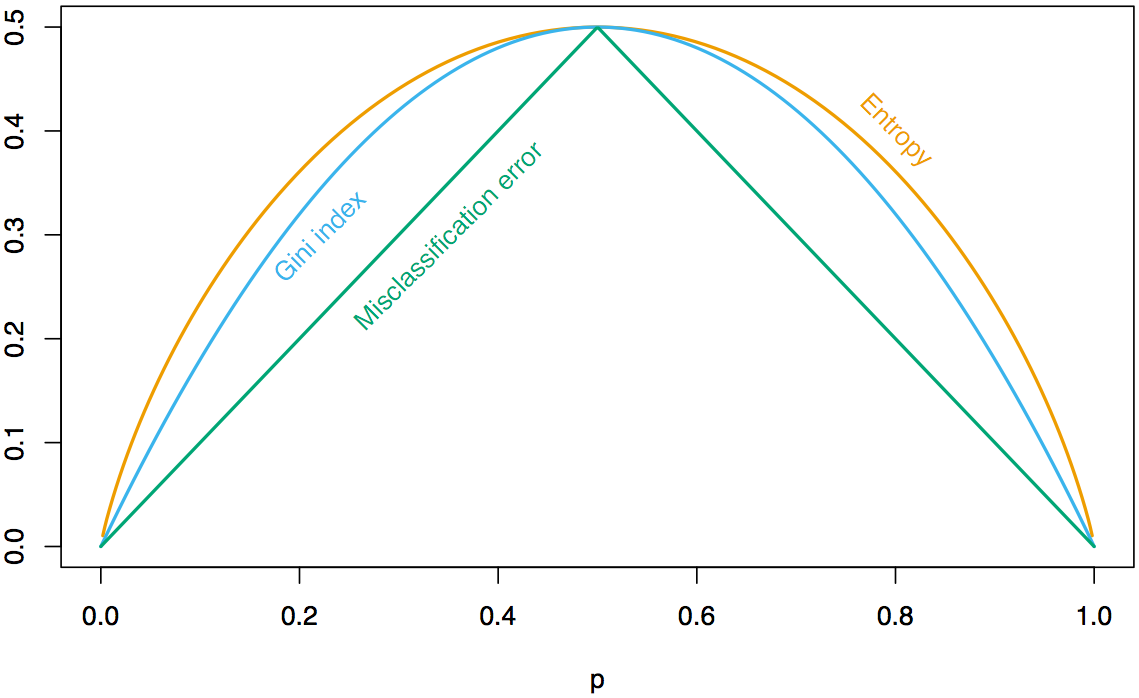
\includegraphics[height=0.5\textheight]{figures/impurityMeasureTwoClass}
\end{figure}
\vspace{-1em}
Misclassification error is not strictly concave thus may not guarantee improvement over the parent node.
\note[item]{On the linear piece of misclassification error,
$w_1Q(p_1) + w_2Q(p_2) = Q(w_1p_1 + w_2p_2)$.}
\let\thefootnote\relax\footnotetext{\tiny{HTF Figure 9.3}}
\end{frame}

\begin{frame}{Finding the Split Point}
How to find a split point that minimizes a given impurity measure?
\begin{itemize}[<+->]
\item<.-> Enumerate $d$ features and $n-1$ split points for each feature.
\item Consider splitting on the $j$'th feature $x_{j}$.
\item If $x_{j(1)},\ldots,x_{j(n)}$ are the sorted values of the $j$'th
feature,
\begin{itemize}[<.->]
\item we only need to check split points between adjacent values
\item traditionally take split points halfway between adjacent values:
\begin{align}
s_{j}\in\left\{ \frac{1}{2}\left(x_{j(r)}+x_{j(r+1)}\right)\mid r=1,\ldots,n-1\right\} .
&& \text{$n-1$ splits}
\end{align}
\end{itemize}
\end{itemize}

\note[item]{Now that we have a measure of goodness for each split. How do we find that split? There are infinitely many split points for each continuous feature.}
\note[item]{But many split points will result in the same regions.}
\end{frame}

\begin{frame}
{Regression trees}
\begin{itemize}
\item Predict the mean value of a node
\begin{align}
k(m) = \text{mean}(y_i \mid x_i \in R_m) .
\end{align}
\item Squared loss as the node impurity measure.
\item Everything else remains the same as classification trees.
\end{itemize}

\note[item]{How do we apply the same splitting strategy for regression problems? What needs to be changed?}
\note[item]{First, instead of predicting the majority class, we predict the mean.}
\note[item]{Impurity is easier---just squared loss, i.e. how much the values deviate from the mean.}
\note[item]{So, to recap, to grow a basic decision tree, we pick an impurity measure and a stopping criterion, start from the root node, then recursively split until a stop criteria is reached. Next, let's consider some practical matters.}
\end{frame}

\subsection{Trees in General}
\begin{frame}
{\dis Categorical features}
\begin{itemize}[<+->]
\item For a categorical feature, we split its values into two groups.
\item<.-> Given a set of categories of size $k$, how many distinct splits? (its power set)
\item Finding the optimal split is \textcolor{red}{intractable} in general.
\item Approximations
\begin{description}[<.->][Numeric encoding]
\item<+->[Numeric encoding] Randomly assign a number to each category
\begin{itemize}
\item Binary classification: proportion of class 0
\item Regression: mean of targets of examples in the category, \ie  \textbf{mean encoding} 
\end{itemize}
\item[One-hot encoding] May grow imbalanced trees, \eg left-branching
\item[Binary encoding] Robust to large cardinality
\end{description}

\item Statistical issues with categorical features
\begin{itemize}[<.->]
\item If a category has a very large number of categories, we can \al{overfit}.
\item Extreme example: Row Number could lead to perfect classification with
a single split.
\end{itemize}
\end{itemize}
\note[item]{One unique characteristic of tree-based models is that they handle categorical features naturally.}
\note[item]{$2^k$ subsets, divided by 2 for symmetry, minus 1 to remove the empty set}
\note[item]{Approximation: we can either reduce it to the continuous case, or reduce the number of categories.
To reduce it to the continuous case, we can randomly assign a number to each category. In binary classification, we can do it slightly smartly by assigning the proportion of negative examples in that category.
To reduce the number of categories, we can use binary encoding, which creates multiple binary features out of one categorical features.}
\note[item]{We should be careful with overfitting with there are a large number of categories though.}
\end{frame}

\begin{frame}
{Interpretability}
\begin{itemize}
\item Trees are certainly easier to explain than other classifiers.
\item Can be used to discover non-linear features.
\item Small trees seem interpretable. For large trees, maybe not so easy.
\item Approximate neural network decision boundaries to gain interpretability
\begin{itemize}
\item Wu M, Hughes M, Parbhoo S, Zazzi M, Roth V, Doshi-Velez F. \href{https://finale.seas.harvard.edu/files/finale/files/beyond_sparcity_tree_regularization_of_deep_01.pdf}{Beyond Sparsity: Tree Regularization of Deep Models for Interpretability}. Association for the Advancement of Artificial Intelligence (AAAI). 2018
\end{itemize}
\end{itemize}
\end{frame}

\begin{frame}
{Trees vs linear models}
Trees have to work much harder to capture linear relations.
\begin{figure}
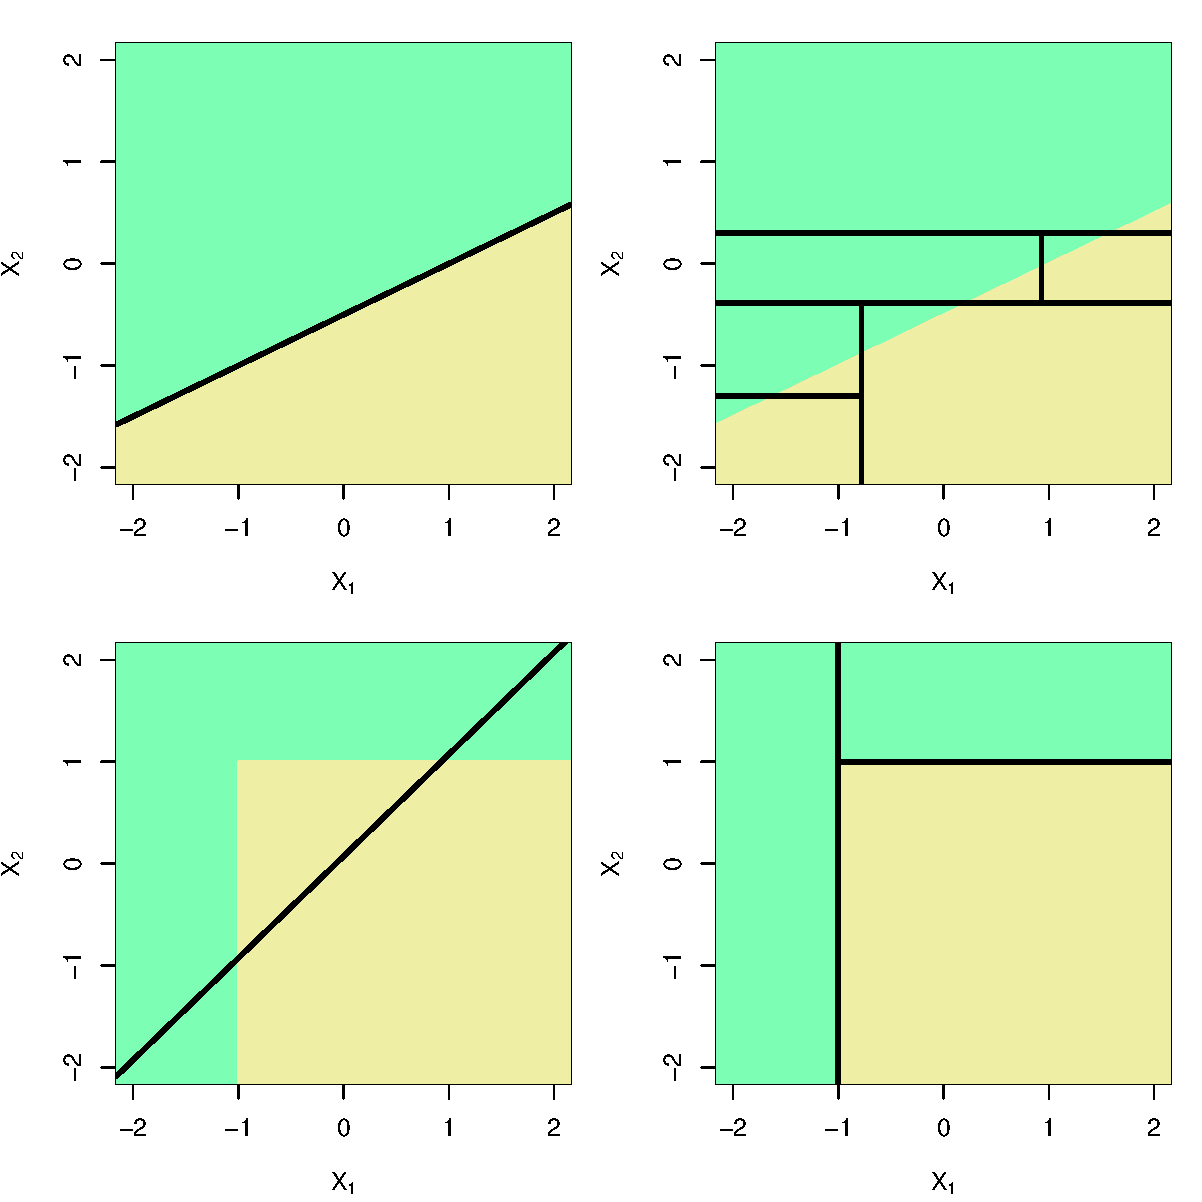
\includegraphics[height=0.6\textheight]{figures/treeVsLinear}
\end{figure}
\note[item]{Because it's hard of it to model the addition of two features.}
\end{frame}

\begin{frame}
{Review}
\begin{simpleblock}{Decision trees:}
\begin{itemize}
\item \emph{Non-linear} classifier that recursively partitions the input space.
\item Non-metric: make no use of geometry, \ie no inner-product or distances.
\item Non-parametric: make no assumption of the data distribution.
\end{itemize}
\end{simpleblock}

\onslide<+->{
\begin{simpleblock}{Pros:}
\begin{itemize}
\item Simple to understand.
\item Interpretable, feature selection for free.
\end{itemize}
\end{simpleblock}
}
\onslide<.->{
\begin{simpleblock}{Cons:}
\begin{itemize}
\item Poor linear modeling.
\item Unstable / high variance, tend to \al{overfit}. $\rightarrow$ Next, how to fix this.
\end{itemize}
\end{simpleblock}
}
\note[item]{What are some pros and cons of trees?}
\note[item]{One big issue with trees is that they are very unstable, meaning that if the training data is changed slightly, our classifier will be quite different, and this makes the performance of a single tree not competitive.}
\end{frame}

\end{document}
